% !TeX encoding = UTF-8
% !TeX spellcheck = en_US

\documentclass[
	ruledheaders=chapter,
	class=report,
	thesis={type=master, department=inf},
	accentcolor=1c,
	custommargins=true,
	marginpar=false,
	parskip=half-,
	fontsize=11pt,
]{tudapub}

\usepackage[english]{babel}

\usepackage[autostyle]{csquotes}
\usepackage{microtype}

\usepackage{enumerate}
\usepackage{enumitem}

\usepackage{biblatex}
\bibliography{thesis-literature}

\usepackage{tabularx}
\usepackage{booktabs}

\usepackage{mathtools}
\usepackage{amssymb}

\usepackage{graphicx}
\usepackage{float}
\usepackage[export]{adjustbox}
\usepackage[font=small,labelfont=bf]{caption}
\graphicspath{ {./images/} }

\counterwithout{footnote}{chapter}

\pagenumbering{roman}

\begin{document}
	\Metadata{
		title=Evaluating the Efficacy of Gaussian Padding on Website Fingerprinting Attacks,
		author=Johannes Leupold
	}
	
	\title{Evaluating the Efficacy of Gaussian Padding on Website Fingerprinting Attacks}
	\author[J. Leupold]{Johannes Leupold}
	\birthplace{Dresden}
	\reviewer{Jean-Paul Degabriele \and Vukasin Karadzic}

	\department{inf}
	\institute{IT Security}
	\group{Cryptography and Network Security}
	
	\submissiondate{01.09.2021}
	\examdate{20.09.2021}
	
	% Hinweis zur Lizenz:
	% TUDa-CI verwendet momentan die Lizenz CC BY-NC-ND 2.0 DE als Voreinstellung.
	% Die TU Darmstadt hat jedoch die Empfehlung von dieser auf die liberalere
	% CC BY 4.0 geändert. Diese erlaubt eine Verwendung bearbeiteter Versionen und
	% die kommerzielle Nutzung.
	% TUDa-CI wird im nächsten größeren Release ebenfalls diese Anpassung vornehmen.
	% Aus diesem Grund wird empfohlen die Lizenz manuell auszuwählen.
	% \tuprints{urn=1234,printid=12345,doi=10.25534/tuprints-1234,license=cc-by-4.0}
	% To see furhter information on the license option in English, remove the license= key and pay attention to the warning & help message.
	
	% \dedication{Für alle, die \TeX{} nutzen.}
	
	\maketitle
	
	\affidavit[digital]% oder \affidavit[digital] falls eine rein digitale Abgabe vorgesehen ist.

	\begin{abstract}[english]
		Abstract
	\end{abstract}
	
	\tableofcontents
	
	\chapter{Introduction}
	\label{introduction}
	\IMRADlabel{introduction}
	\pagenumbering{arabic}

	This is the introduction.

	\chapter{Background Material}
	\label{fingerprinting}

	\section{Theoretical Setting}
	\label{theoretical}
	
	Website Fingerprinting (WF) is a field of study focusing on data leaked from anonymization 
	techniques and whether it is still sufficient to conclude which websites the user visited.
	Furthermore, a goal of Website Fingerprinting study is the evaluation of various countermeasures
	that limit the leaked data and thus thwart attempts to uncover the websites a certain user was
	visiting.
	
	\subsection{Threat Model}
	\label{theoretical:threat_model}
	
	The Website Fingerprinting adversary is assumed to have access to the encrypted network traffic of the victim. However, he is not able to decrypt the traffic, or parts of it, so he can only draw conclusions based on metadata of the encrypted packets. In particular, the adversary observes 
	
	\begin{itemize}
		\item packet length (full packet size in bytes),
		\item direction (whether the packet goes from Client $\to$ Server, or vice versa), and
		\item timing (amount of time between the first packet and the current packet).
	\end{itemize}

	This information also gives way to various derived measures, such as overall bandwidth consumed, overall time, or burst\footnote{A \textit{burst} is a contiguous sequence of packets going in the same direction} length/size.
	
	Before the adversary begins with the attack, he can create a database of websites the victim may visit and collect so-called \textit{packet traces} for the websites. A packet trace is a sequence $\mathcal{T} = \langle p_1,p_2,...,p_n\rangle$ of tuples $p_i = (t_i, l_i, d_i) \in \mathbb{N} \times \{52, \ldots, MTU\} \times \{\uparrow, \downarrow\}, i = 1,\ldots,n$, where $t_i$, $l_i$ and $d_i$ denote the time, length and direction for a single observed packet, respectively. The packet length can never be smaller than 52 bytes, as that is the size of the smallest possible TCP/IP packet, the ACK packet. The maximum packet size $MTU$ (also called \textit{Maximum Transmission Unit}) is dependent on the used network technologies. For Ethernet, the MTU is 1500 bytes, while for WiFi (IEEE 802.11) it is 2312 bytes. Note that the adversary is assumed to collect his database of website traces under the same technical preconditions (network technologies) that his victim uses to access them. When carrying out the attack, the adversary observes packet traces for particular page loads of the victim. He may then use any algorithm and his prepared database to try and deduce which websites out of the pre-selected set the victim visited. When a WF countermeasure is in place, the adversary is assumed to be aware of it such that he can collect his trace database under the same countermeasure.
	
	\subsection{Attacks and Countermeasures}
	\label{theoretical:attacks_and_defenses}
	
	To successfully make conclusions on the websites a victim visited, the attacker needs to classify the packet traces he observed to be an instance of one of the websites in his database. He may achieve this by randomly guessing the instance's class, but this naive method can't be expected to yield good results for higher numbers of websites. Therefore, the adversary may employ a Machine Learning technique, consisting of a feature extraction\footnote{\textit{Feature Extraction} refers to transforming a certain observation into a number of (mostly numerical) attributes, called \textit{features}} and a classification algorithm. A classification algorithm is trained using a number of examples from all classes including the class labels (the \textit{training set}). In the following, an overview of common classification algorithms is given.
	
	\begin{description}
		\item[Nearest Neighbours] The Nearest Neighbours classifier (also called NN) is a simple algorithm that assigns to each instance the class of its nearest neighbor according to some distance metric. It may be extended to $k$-Nearest-Neighbours (kNN) by considering the nearest $k$ neighbors and taking the majority vote of their classes. One may also apply weighting to the neighbors based on the distance from the point to be classified.
		\item[Naive Bayes] The Naive Bayes classifier tries to estimate probability distributions for the attribute values conditioned on all classes from the training data. It estimates the probability distributions $p(C)$ and $p((f_1, ..., f_k) \mid C)$ from the data for all classes $C$ and attribute values $f_1, ..., f_k$. To classify a new example e $(g_1, ..., g_k)$, Bayes' rule is used to calculate $p(C \mid (g_1, ..., g_k))$ for each class $C$ and the class yielding the highest probability is returned. The method used to estimate the probability distributions from the data can be chosen according to the requirements of the problem. Common examples include simply fitting a normal distribution using a maximum likelihood approach, and Kernel Density Estimation (see below).
		\item[Kernel Density Estimation (KDE)] The term "Kernel Density Estimation" refers to a method used to estimate the underlying probability density function a certain set of samples was drawn from. To this end, individual functions, called \textit{kernels} are centered at each sample. To evaluate the density function at a certain point, all individual kernels are evaluated and summed up. Equation \ref{eq:kde} shows the general formula with $n$ being the number of training samples, $k$ being the kernel function and $h$ being a parameter called \textit{bandwidth} that controls smoothing.
		\begin{equation}
			\label{eq:kde}
			p(x) = \frac{1}{nh}\sum_{i = 1}^{n} k\left(\frac{x - x_i}{h}\right)
		\end{equation}
		A common choice for $k$ is the standard normal density function.
		\item[Support Vector Machine (SVM)] The SVM is a sophisticated classification algorithm trying learn a hyperplane to separate the examples of different classes in the feature space. This is achieved by selecting the hyperplane that yields the largest separation between the classes, i.e. the one that maximizes the distance to the nearest points of each class. Support Vector Machines are well suited for working with high-dimensional feature spaces and may use a non-linear transformation of data points into an implicit higher-dimensional feature space. This transformation is called a \textit{kernel} (not to be confused with the kernel used in Kernel Density Estimation). \cite{Boser1992,Cortes1995}
	\end{description}

	A defense against WF attacks aims at disguising the identifying patterns in the packet traces the attacker can observe. To this end, packets lengths may be artificially changed, they may be split up into multiple packets, or the timing might be changed. There exist three main classes of defenses, while, naturally, some countermeasures might not fit one particular class, but exhibit characteristics of multiple classes.
	
	\begin{description}
		\item[Padding] Padding schemes are among the simplest countermeasures. They add certain amounts of dummy data to each packet up to the MTU. Padding schemes may be \textit{deterministic} or \textit{randomized}, with deterministic schemes always returning the same output trace when presented the same input trace, while this isn't the case for randomized padding. When using this type of defense, packets can only grow, but never shrink. Also, packet counts and timing are not affected.
		\item[Noise] Defenses of this class try to disguise the visited web page by deliberately adding noise to the transmission. This can be done for example by loading a second randomly chosen web site in parallel to the requested site \cite{Panchenko2011} or randomizing the order of HTTP requests in the web browser \cite{Perry2011}. Countermeasures using approach may affect packet timing and order and insert new packets into the trace.
		\item[Morphing] Morphing countermeasures are the most complex defenses, trying to hide the actual distribution of packet sizes. They may simply try to make all websites look equal, or at least similar, \cite{Dyer2012,Cai2014,Cai2014a} or to make a certain web site look like a different one \cite{Wright2009}. Packet traces may be changed in many ways when using a morphing defense, like adding extra packets, growing or splitting packets, or changing timing.
	\end{description}
	
	\section{Gaussian Padding}
	\label{gaussian_padding}
	
	\textit{Gaussian padding} is a specific form of randomized padding. The amount of dummy data added to a packet is drawn from a rounded normal distribution, as opposed to Uniform Padding, where padding sizes are drawn according to the uniform distribution. Furthermore, the tails of the distribution are clipped on both sides, as padding can never take negative values and packets may never become bigger than the MTU. The distribution is parameterized with the desired mean padding size, becoming the mean $\mu$ of the normal distribution. The standard deviation $\sigma$ can be chosen such that the truncated tail corresponds to as little probability mass as desired. For our purpose, choosing $\sigma = \frac{\mu}{3}$ is sufficient, as in this case only approximately $0.1\%$ of the probability mass is allocated to negative values. Figure \ref{fig:trunc_gauss} shows an example distribution function for a truncated rounded normal distribution.
	
	Sampling from a rounded normal distribution is straight-forward by simply sampling from a continuous normal distribution and rounding the value. The truncation can be achieved by rejecting and resampling values that fall out of the desired interval, or by using the method described by Hülsing et al. in \cite{Huelsing2018}, which allows to sample from a rounded Gaussian in constant time, thus mitigating cache timing attacks on the sampling algorithm. While these are out of scope under the threat model of WF, this fact is of particular interest for different fields of research, such as Lattice-based cryptography. \cite{Huelsing2018}
	
	When applying Gaussian padding, the amount of data added to each packet may either be sampled from the distribution independently for each individual packet or once for every session (i.e. page load), leading to \textit{packet-random} Gaussian padding and \textit{session-random} Gaussian padding, respectively.
	
	\begin{figure}[tb]
		\centering
		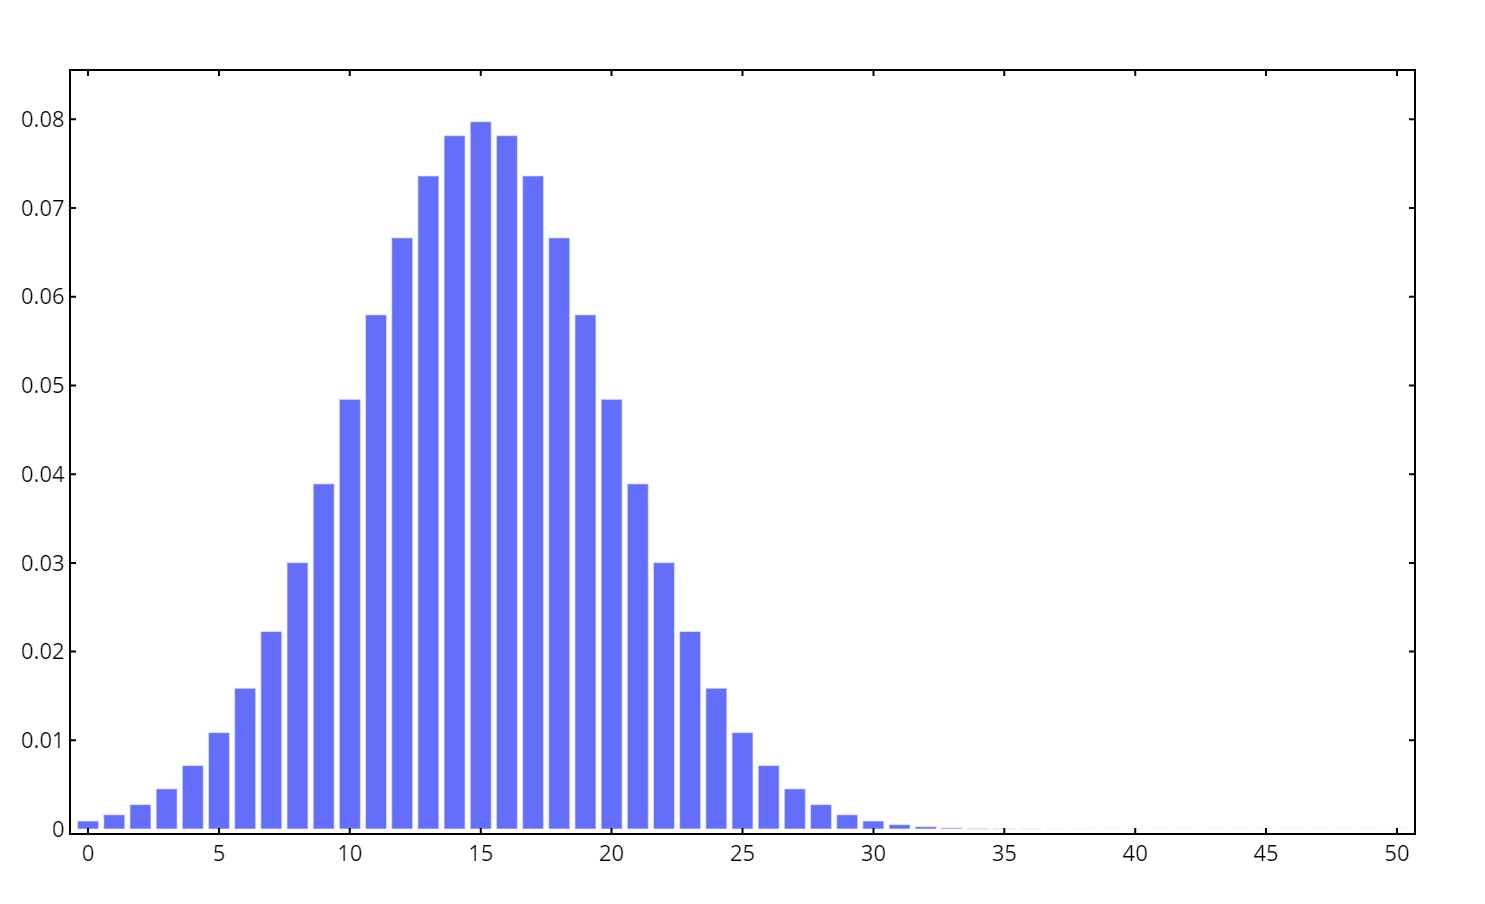
\includegraphics[width=\textwidth]{truncated_rounded_normal.png}
		\caption{An example for a rounded normal distribution, truncated to the left at 0 with a mean padding size of $\mu = 15$ and a standard deviation of $\sigma = 5$ }
		\label{fig:trunc_gauss}
	\end{figure}
	
	\section[Security Bound Estimation]{Security Bound Estimation According to Cherubin \cite{Cherubin2017}}
	\label{cherubin_bounds}
	
	When evaluating WF attacks and defenses, the traditional approach is to empirically measure their performance on a previously collected data set of packet traces. However, such empirical
	evaluations are susceptible to noise and fail to produce provable statements on the security of
	a certain defense. While a defense may perform particularly well against the attacks it is evaluated on, it may just as well horribly fail on a different attack that wasn't considered yet. To address this problem and further advance research on provable security evaluation of WF defenses, Cherubin introduces a novel method centered around the Bayes error in \cite{Cherubin2017}.
	
	The \textit{Bayes error} is defined as the minimum probability of error that any classifier can commit given a joint probability distribution on the features and class labels.  Intuitively speaking, the Bayes error corresponds to the area of uncertainty in the probability distribution, i.e. the area where the conditional probabilities $p(x \mid c_i)$ and $p(x \mid c_j)$ overlap\footnote{That is, both probabilities are non-zero} for any two classes $c_i \neq c_j$ and features $x$. 
	
	To formalize, let $\mathcal{X}$ be the feature space and $\mathcal{C}$ the set of all class labels. Let $p(x, c)$ be a joint probability distribution on $\mathcal{X}\times\mathcal{C}$. Then for the set of classifiers $\mathcal{F} = \{f \mid f : \mathcal{X} \to \mathcal{C}\}$ with $R_f$ being the error of a classifier $f\in\mathcal{F}$ according to $p$, the Bayes error $R^*$ is defined as
	
	\begin{align}
		R^* &= \min_{f\in\mathcal{F}} R_f
		\intertext{This minimum error is achieved by the \textit{Bayes classifier} $f^*\in\mathcal{F}$ that assigns to each example $x$ the class label $c$ maximizing the probability $p(c \mid x)$ \cite{Duda2000}.}
		f^*(x) &= \arg\max_{c\in\mathcal{C}} p(c \mid x) \\
		R^* &= R_{f^*}
	\end{align}

	As the true joint probability distribution $p(x, c)$ is typically not known in practice, the exact value of the Bayes error can't be calculated. However, there are well-known methods to estimate a lower bound for the Bayes error. Cherubin uses an estimate based on the NN classifier (see section \ref{theoretical:attacks_and_defenses}) first presented by Cover and Hart \cite{Cover1967} deriving a lower bound $\widehat{R}^*$ for the Bayes error $R^*$
	
	\begin{equation}
		\widehat{R}^* = \frac{L - 1}{L} \left(1 - \sqrt{1 - \frac{L}{L-1}\widehat{R}_{NN}}\right) \leq R^*
	\end{equation}

	where $\widehat{R}_{NN}$ is the empirical error of the NN classifier on a data set containing $L = |\mathcal{C}|$ classes

	\chapter{Prior Work}
	\label{related}

	\chapter{Experimental Methodology}
	\label{methods}
	\IMRADlabel{methods}

	\section{Trace Data}
	\label{dataset_quality}

	\section{Evaluating Attack Performance}
	\label{pipeline}

	\section{Error Bound Estimation}
	\label{error_bound_estimation}

	\chapter{Results}
	\label{results}
	\IMRADlabel{results}

	\section{Empirical Performance of Gaussian Padding}
	\label{performance}

	\section{Estimated Security Bounds}
	\label{security_bounds}

	\chapter{Discussion}
	\label{discussion}
	\IMRADlabel{discussion}

	\chapter{Conclusion}
	\label{conclusion}

	\pagebreak
	\pagenumbering{roman}
	\setcounter{page}{5}
	\addcontentsline{toc}{chapter}{Bibliography}
	\printbibliography

	\cleardoublepage
	\phantomsection
	\addcontentsline{toc}{chapter}{\listfigurename}
	\listoffigures

	\cleardoublepage
	\phantomsection
	\addcontentsline{toc}{chapter}{\listtablename}
	\listoftables
\end{document}